\documentclass[spanish,12pt, a4paper, twoside]{paper}

\let\oldsection\section
\def\section{\cleardoublepage\oldsection}

\usepackage{afterpage}

\newcommand\blankpage{%
    \null
    \thispagestyle{empty}%
    \addtocounter{page}{-1}%
    \newpage}

\usepackage[textwidth=15cm, textheight=22.5cm, top=3.5cm, bottom=3.5cm,left= 4cm,right=2cm]{geometry}


\usepackage[spanish]{babel}
%\usepackage[applemac]{inputenc} 
%POR DEFECTO SE ESTÁ USANDO EL PAQUETE PARA RECONOCER ACENTOS DE MAC, EN CASO DE USAR WINDOWS COMO SISTEMA OPERATIVO ELIMINAR LA LÍNEA ANTERIOR E INTRODUCIR LA SIGUIENTE
\usepackage[utf8]{inputenc}

\usepackage{graphicx}
\usepackage{graphics}
\usepackage{amsmath,amssymb}
\usepackage{float}
\usepackage{changepage}
\usepackage{subcaption}


\usepackage{algorithm}
\usepackage{multirow}


\begin{document}
%\maketitle
%\thispagestyle{empty}
\begin{titlepage}

\newcommand{\HRule}{\rule{\linewidth}{0.5mm}} % Defines a new command for the horizontal lines, change thickness here

\center % Center everything on the page
 
%	HEADING SECTIONS

\includegraphics[width=4cm]{recursos/logoEtsisi.png}
  \hspace{8cm}

\includegraphics[width=2cm]{recursos/logo.png}
\\[1cm]

\textsc{\Large Escuela Técnica Superior de Sistemas Informáticos}\\[0.5cm]
\textsc{\large Universidad Politécnica de Madrid}
\\[3cm]


%	TITLE SECTION
 \HRule \\[0.4cm]
{ \huge \bfseries BFMB: Framework Base para Bots Modulares}\\[0.4cm] % Title of your document
\HRule \\[2.5cm]

\textsc{\LARGE Trabajo Fin de Grado}\\[0.5cm] 
\textsc{\Large Grado en Ingeniería del Software }\\[2.5cm]

 %	AUTHOR SECTION
\begin{flushright}
\large
AUTOR: Ángel González Abad\\
TUTOR: Dr. Francisco Javier Gil Rubio
\end{flushright}

\vspace{1.3cm}

%	DATE SECTION
{ {2018}}\\[3cm]
%	LOGO SECTION

\vfill % Fill the rest of the page with whitespace

\end{titlepage}

\afterpage{\blankpage}
\pagenumbering{roman}


%	AGRADECIMIENTOS
\section*{AGRADECIMIENTOS}
Aquí estarán los agradecimientos cuando se me ocurra que poner.

%	RESUMEN
\section*{RESUMEN}
Extensión máxima de una página


%	SUMMARY
\section*{SUMMARY}
Extensión máxima de una página


%	ÍNDICE
\tableofcontents % indice de contenidos



%	INDICE DE FIGURAS Y TABLAS
\listoffigures
\listoftables



%	CAPÍTULOS DEL TRABAJO FIN DE MÁSTER
\newpage
\pagenumbering{arabic} 

\section{INTRODUCCIÓN Y OBJETIVOS}

\noindent Aquí he de hablar sobre cómo comenzó todo esto y porqué.

\section{ESTADO DEL ARTE}

\noindent Aquí toca hablar sobre la historia de los chatbots, su progreso y su situación actual.

\section{ANÁLISIS}



\section{DISEÑO Y ARQUITECTURA DEL SISTEMA}

\subsection{Casos de uso}

\begin{figure*}
\centering
	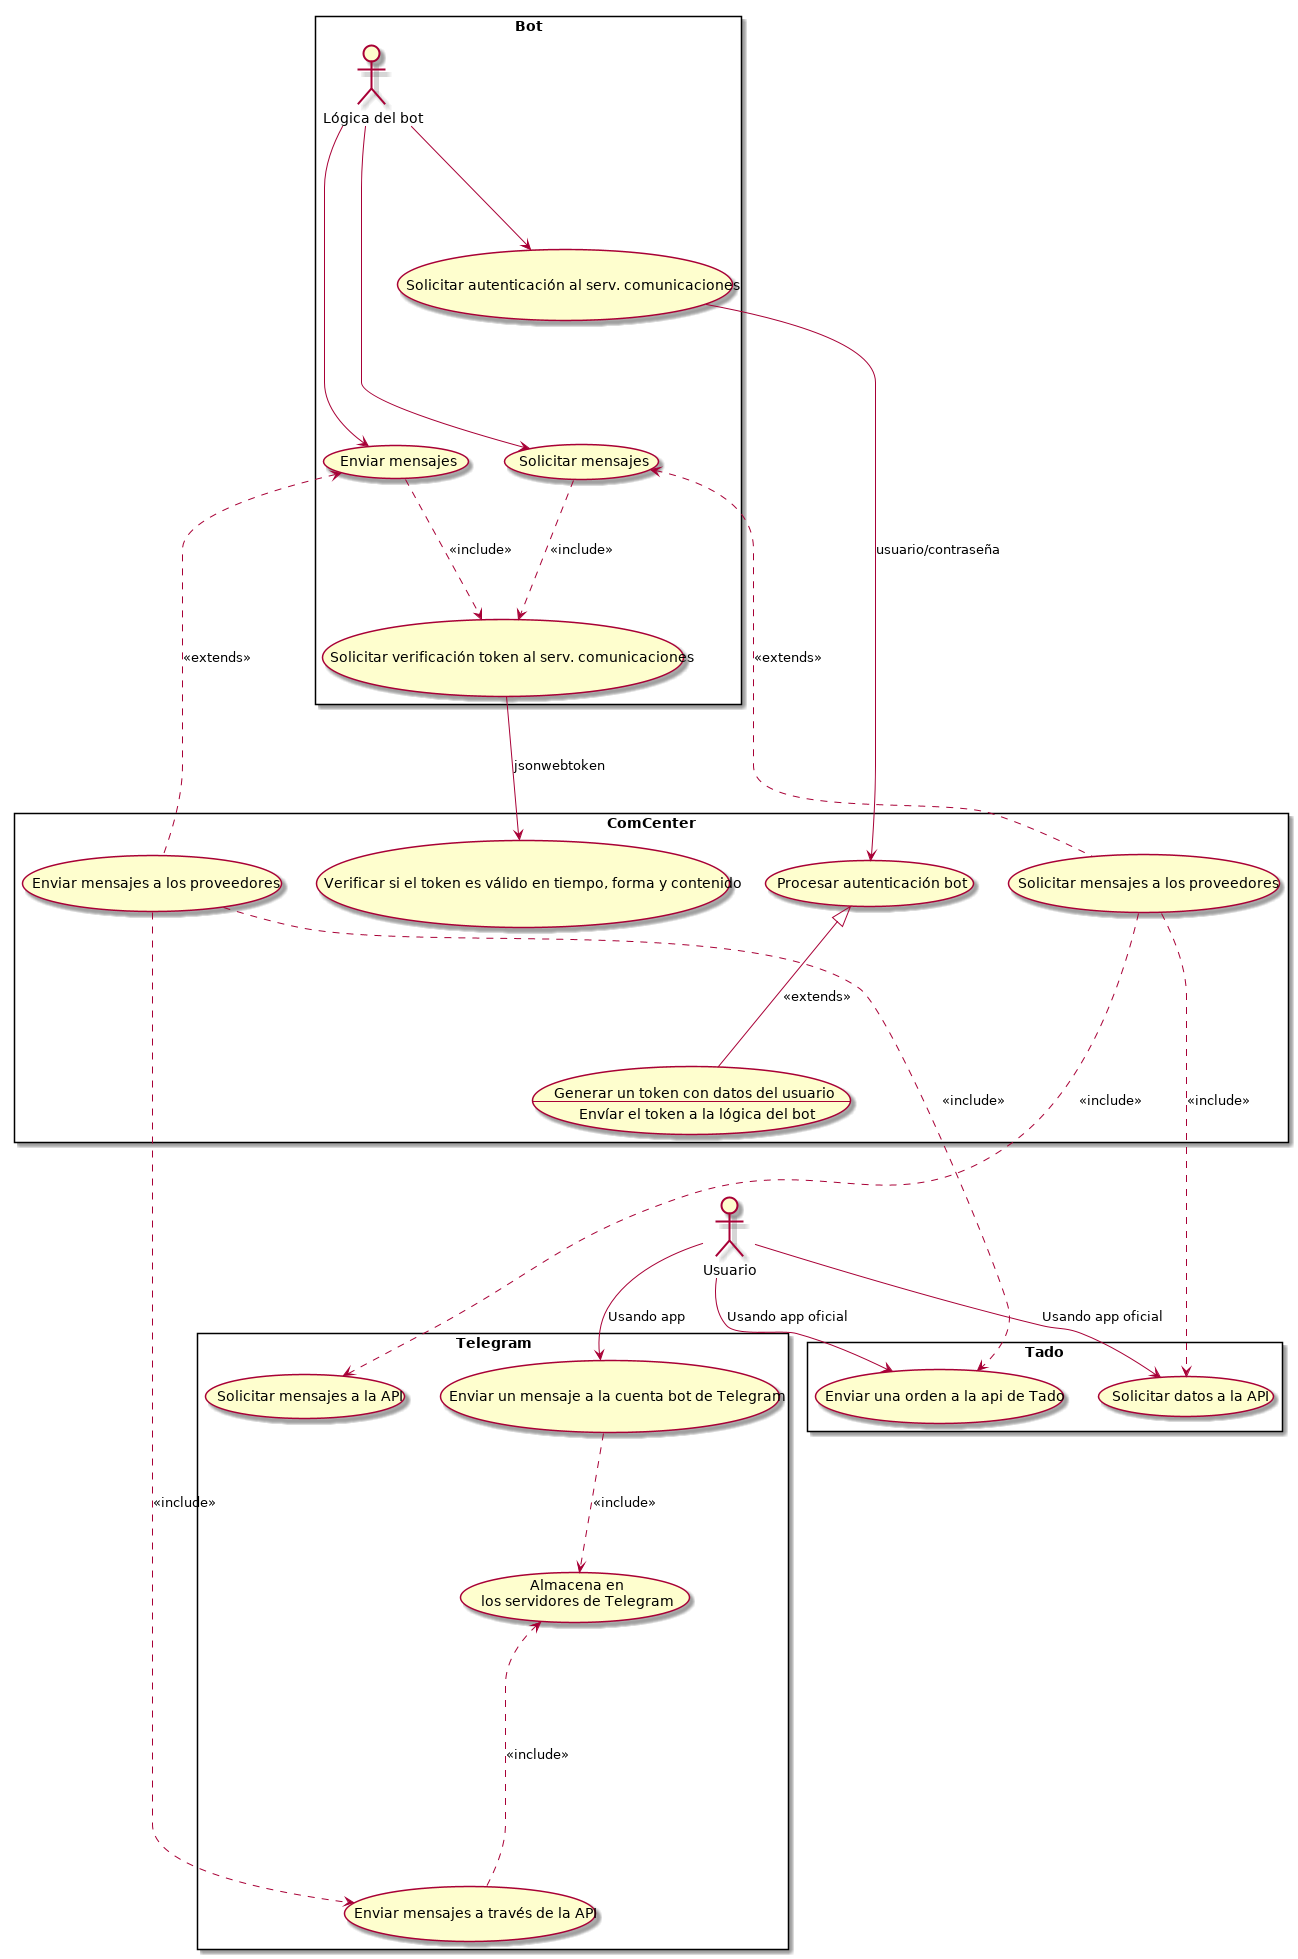
\includegraphics[width=\textwidth]{recursos/usecases}
\caption{Diagrama de casos de uso}
\label{fig:Diagrama de casos de uso}
\end{figure*}

\subsection{Infraestructura}

\begin{figure*}
\centering
	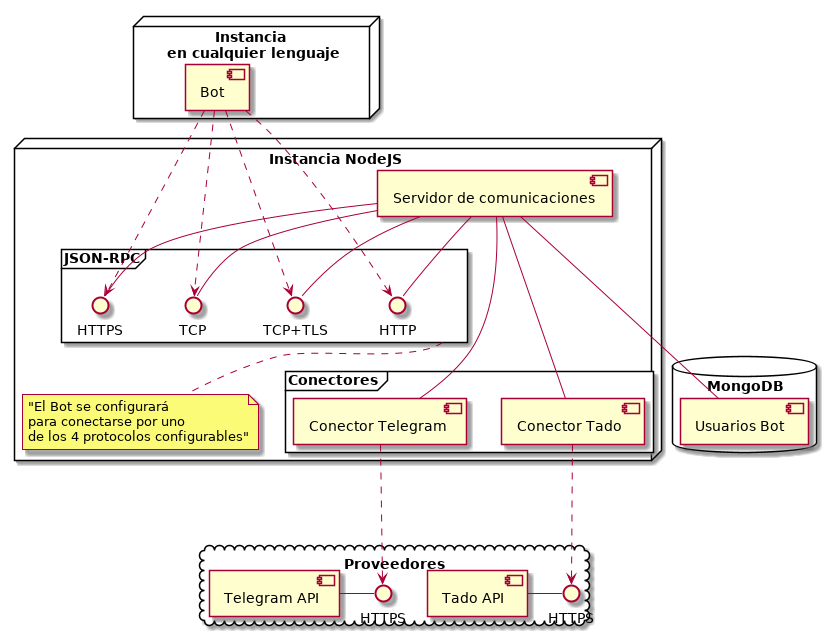
\includegraphics[width=\textwidth]{recursos/component}
\caption{Esquema de infraestructura (Diagrama de componentes)}
\label{fig:Infraestructura de nodos}
\end{figure*}

\subsection{Estructura de base de datos}

\subsection{Disposición del código}

\begin{figure*}
\centering
	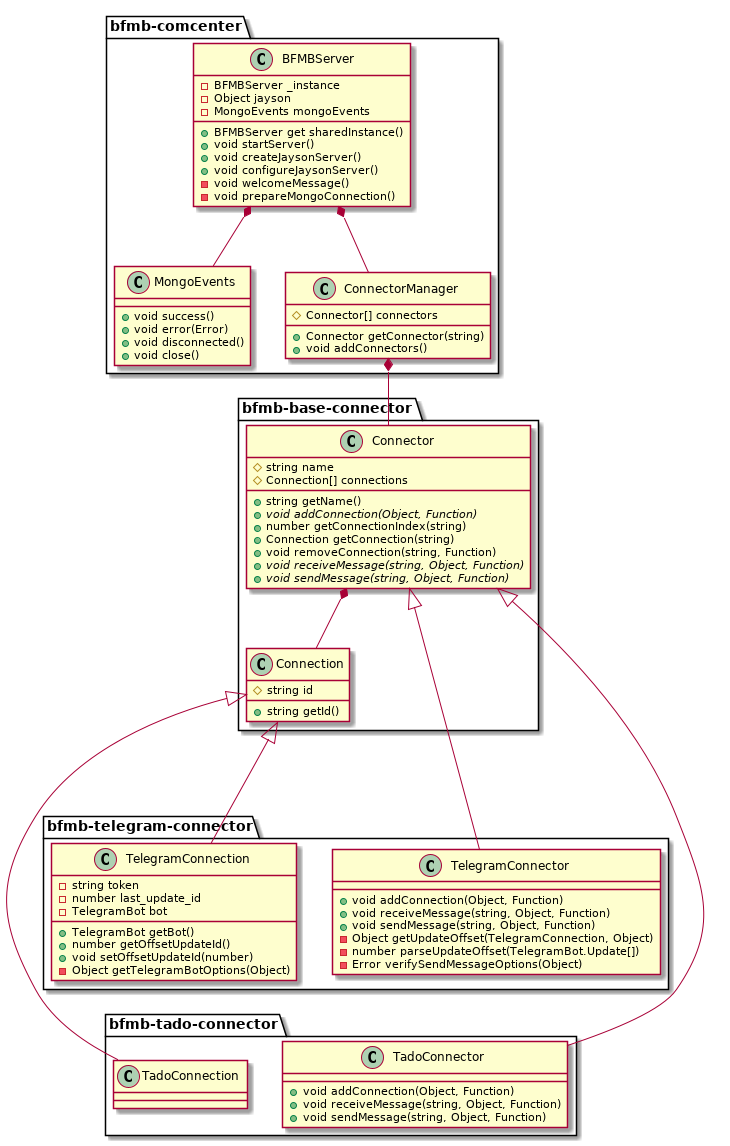
\includegraphics[width=\textwidth]{recursos/classes}
\caption{Diagrama de clases}
\label{fig:Diagrama de clases}
\end{figure*}

\section{DESARROLLO}

\subsection{Lenguaje de desarrollo}

\subsection{Dependencias}

\subsubsection{Software externo}

\subsubsection{Bibliotecas}

\subsubsection{Servicios externos}

\section{PRUEBAS}

\section{MANUAL DE USUARIO}

\section{CONCLUSIONES}

\section{LÍNEAS FUTURAS}

\section{TABLAS, FIGURAS, EXPRESIONES MATEMÁTICAS Y ALGORITMOS}

\subsection{Figuras}

Las Figuras \ref{fig:Bernoulli1} y \ref{fig:violin_besa_escenario4} muestran ejemplos de cómo insertar figuras en el TFM.



\subsection{Expresiones matemáticas}
A continuación, se muestran algunos ejemplos de expresiones matemáticas:
\begin{equation}
\mu^*\times 25000-\frac{1}{1000}\sum_{r=1}^{1000}\sum_{i=1}^{K}\sum_{j=1}^{25000}\mu_i\times X_{i,j}^r.
\end{equation}

\begin{equation}
\mu_{\widetilde{A}}(x)=\left\{ \begin{array}{cc}
\frac{x-a_{1}}{a_{2}-a_{1}} & if\; a_{1}\leq x\leq a_{2}\\
1 & if\; a_{2}\leq x\leq a_{3}\\
\frac{x-a_{4}}{a_{3}-a_{4}} & if\; a_{3}\leq x\leq a_{4}\\
0 & otherwise
\end{array}\right. .
\end{equation}


\begin{equation}
\begin{tabular}{ll}
$\widetilde{DD}(A_{1},A_{4})$ & $=\widetilde{DD}(A_{1},A_{4}|P_{1})\oplus 
\widetilde{DD}(A_{1},A_{4}|P_{2})$ \\ 
& $=[\widetilde{dd}(A_{1},A_{2})\otimes \widetilde{dd}(A_{2},A_{4})]\oplus \lbrack \widetilde{dd}(A_{1},A_{3})\otimes \widetilde{%
dd}(A_{3},A_{4})].$%
\end{tabular}%
\end{equation}



\begin{itemize}
\item Si$\;{max} \{(a_{4}-a_{1}),(b_{4}-b_{1})\}\neq 0$, entonces
\begin{eqnarray*}
{\small S(}\widetilde{A}{\small ,}\widetilde{B}{\small )} &{\small =}&%
\left. {\small 1-(1-\alpha -\beta })\times \left ( {\small 1-}\frac{\int_{0}^{1}%
{\small \mu }_{\widetilde{A}\cap \widetilde{B}}{\small (x)dx}}{\int_{0}^{1}%
{\small \mu }_{\widetilde{A}\cup \widetilde{B}}{\small (x)dx}}\right)
\right.  \\
&&\left. -{\small \alpha } \frac{\sum {\small \mid a}_{i}{\small -b}_{i}%
{\small \mid }}{{\small 4}}-{\small \beta }\frac{{\small d[(X}_{\widetilde{A}%
}{\small ,Y}_{\widetilde{A}}{\small ),(X}_{\widetilde{B}}{\small ,Y}_{%
\widetilde{B}}{\small )]}}{{\small M}}\right., 
\end{eqnarray*}

\item En caso contrario,%
\begin{eqnarray*}
{\small S(}\widetilde{A}{\small ,}\widetilde{B}{\small )} &{\small =}&%
\left. {\small 1-}%
\left( \frac{{\small 1-\alpha -\beta }}{{\small 2}}{\small +\alpha } \right) \times
\frac{\sum {\small \mid a}_{i}{\small -b}_{i}{\small \mid }}{{\small 4}}%
{\small -}\right.  \\
&&\left. {\small -}\left( \frac{{\small 1-\alpha -\beta }}{{\small 2}}%
{\small +\beta }\right)\times \frac{{\small d[(X}_{\widetilde{A}}{\small ,Y}_{%
\widetilde{A}}{\small ),(X}_{\widetilde{B}}{\small ,Y}_{\widetilde{B}}%
{\small )]}}{{\small M}}\right., 
\end{eqnarray*}
\end{itemize}
donde $\alpha +\beta <1$, $\mu _{\widetilde{\chi }}$ es la función de pertenencia de $\widetilde{\chi}$, 
\begin{equation}
M=\underset{[0,1]\times[0,\frac{1}{2}]}{max}\{d((x,y),(x^{\prime },y^{\prime }))\}\text{,} 
\end{equation}%
\begin{equation*}
\mu _{\widetilde{A}\cap \widetilde{B}}(x)=\underset{0\leq x\leq 1}{min}%
\{\mu _{\widetilde{A}}(x),\mu _{\widetilde{B}}(x)\} ,
\;\;\; \mu _{\widetilde{A}\cup \widetilde{B}}(x)=\underset{0\leq x\leq 1}{max}%
\{\mu _{\widetilde{A}}(x),\mu _{\widetilde{B}}(x)\}.
\end{equation*}%

\subsection{Algoritmos}

El Algoritmo \ref{getDelay} ilustra la forma que debe adoptarse. 
\begin{algorithm}[h]
%\begin{algorithmic}
{\bf  Data:} ($t_0$ = instante en el que se genera el retardo)
\medskip

\hspace{0.5em} {\bf if} $(update\_architecture==1)$ {\bf then} 

\hspace{1.5em} {\bf if} $(delay\_scenario==1)$ {\bf then} delay$=C$

\hspace{1.5em} {\bf else} 

\hspace{2.5em} {\bf if} $(reward\_scenario==1)$ {\bf then} 

\hspace{3.5em} delay $\leftarrow [0,300]$-trunc\_Exp($\lambda=1/80$)

\hspace{2.5em} {\bf else} 

\hspace{3.5em} delay $\leftarrow [0,480]$-trunc\_Exp($\lambda=1/150$)

\hspace{2.5em} {\bf end if}

\hspace{1.5em} {\bf end if}

\hspace{0.5em} {\bf else} (arquitectura en modo batch)

\hspace{1.5em} delay= difference(24:00, $t_0$)

\hspace{0.5em} {\bf end if}

\hspace{0.5em}  {\bf return} delay

{\bf end} 
\caption{$getDelay(t_0)$}
\label{getDelay}
\end{algorithm}


\subsection{Tablas}
Las Tablas \ref{table:results45} y \ref{table:risk} muestran el formato de tabla a utilizar.

\begin{table}[htb]
\centering
\caption{Mean cumulative regrets and standard deviations}
\label{table:results45}
\begin{tabular}{llllll}
\hline
 & \multicolumn{2}{c}{\small Truncated Poisson} &  & \multicolumn{2}{c}{\small Truncated Exponential} \\ 
\cline{2-3}\cline{5-6}\cline{5-6}
  & {\small Mean} & ${\small \sigma}$ &  &  {\small Mean} & ${\small \sigma}$\\ \hline
 {\small UCB}      & {\small 2632.65} & {\small 246.03}  &  & {\small 1295.79} & {\small 514.03}   \\
 {\small DMED+}            & {\small 978.56} & {\small 225.24}  &  & {\bf \small645.70} & {\small 493.8}   \\
  {\small KL-UCB}   & {\small 1817.4} & {\small 236.57}  &  & {\small 1219.98} & {\small 510.69}   \\ 
  {\small KL-UCB poisson}    & {\bf \small314.99*} & {\small 201.79}  &  & {\small -} & {\small -}   \\
  {\small KL-UCB exp}    & {\small -} & {\small -}  &  & {\small 786.30} & {\small 498.16}   \\
  {\small KL-UCB+}    & {\small 1190.64} & {\small 225.82}  &  & {\small 813.45} & {\small 494.59}   \\
 {\small BESA}      & {\small 2015.73} & {\small 3561.5}  &  & {\small 755.87} & {\small 2323.22}   \\
 {\small PR-1}            & {\small 1314.9} & {\small 234.25}  &  & {\small 660.64} & {\small 492.37}   \\ 
 {\small PR-2 (TS)}  & ${\bf 917.67}$ & {\small222.79}  &  & {\bf \small630.38} & {\small487.01} \\
 {\small PR-3}  & ${\bf 736.6}$ & {\small210.96}  &  & {\bf \small565.79*} & {\small480.99} \\
\hline
\end{tabular}
\end{table}

\begin{table}[htb]
\centering
\caption{Risks to $A_5$ after the implementation of the selected safeguards }
\label{table:risk}
\begin{tabular}{cccc}
\hline
\noalign{\smallskip} 
 {\scriptsize{Threat}}& {\scriptsize{Confidentiality}} & {\scriptsize{Integrity}} & {\scriptsize{Authenticity}}\tabularnewline
\hline  
{\scriptsize{$T_{1}^{1}$}} & \scriptsize{(16.9, 161.72, 936.2, 3681.5)} & \scriptsize{(32.70, 239.7, 1295.6, 5197.4)} & \scriptsize{(25.1, 198.6, 1576.7, 5777.1)}\\
{\scriptsize{$T_{1}^{2}$}} & \scriptsize{(0, 49.6, 458.1, 1791.2)} & \scriptsize{(0, 29.7, 289.7, 1397.1)} & \scriptsize{(0, 24.6, 352.6, 1552.9)}\\
{\scriptsize{$T_{2}^{2}$}} & \scriptsize{(0, 49.6, 458.1, 1791.2)} & \scriptsize{(0, 29.7, 289.7, 1397.1)} & \scriptsize{(76, 379.3, 2074.3, 5588.4)}\\
{\scriptsize{$T_{1}^{3}$}} & \scriptsize{(12.2, 110.5, 647.2, 2465.6)} & \scriptsize{(21.9, 147.3, 744.3, 2958.7)} & \scriptsize{(6.8, 58.5, 487.1, 1923.2)}\\ 
{\scriptsize{$T_{1}^{4}$}} & \scriptsize{(34.8, 245.5, 1176.8, 3793.2)} & \scriptsize{(62.7, 327.4, 1353.3, 4551.9)} & \scriptsize{(19.5, 129.9, 885.7, 2958.7)}\\
\hline 
\end{tabular}
\end{table}



\section{SOBRE LAS REFERENCIAS}

La bibliografía o referencias deben aparecer siempre al final de la tesis, incluso en aquellos casos donde se hayan utilizado notas finales. La bibliografía debe incluir los materiales utilizados, incluida la edición, para que la cita pueda ser fácilmente verificada. 

\bigskip
{\bf Citar dentro del texto:}

Las fuentes consultadas se describen brevemente dentro del texto y estas citas cortas se amplían en una lista de referencias final, en la que se ofrece la información bibliográfica completa. 

La cita dentro del texto es una referencia corta que permite identificar la publicación de dónde se ha extraído una frase o parafraseado una idea, e indica la localización precisa dentro de la publicación fuente. Esta cita informa del apellido del autor, la fecha de publicación y la página (o páginas) y se redacta de la forma que puede verse a través de los siguientes ejemplos:

Cuando se citan las palabras exactas del autor deben presentarse entre comillas e indicarse, tras el apellido del autor y, entre paréntesis, la fecha de publicación de la obra citada, seguida de la/s página/s.

Si lo que se reproduce es la idea de un autor (no sus palabras exactas) no se pondrán comillas y se indicará, entre paréntesis, el apellido del autor seguido de la fecha de publicación de la obra a la que se refiere.

No se puede eliminar una parte del texto citado sin señalarse; debe indicarse siempre con puntos suspensivos entre corchetes [...]

Ejemplos de como citar una referencia en el texto son los siguientes \cite{Ashtiani2014} o \cite{Ashtiani2014,Mateos2009,Vicente2016}.


\bigskip
{\bf Cómo ordenar las referencias:}
\begin{enumerate}
\item Las referencias bibliográficas deben presentarse ordenadas alfabéticamente por el apellido del autor, o del primer autor en caso de que sean varios.
\item Si un autor tiene varias obras se ordenarán por orden de aparición.
\item Si de un mismo autor existen varias referencias de un mismo año se especificarán los años seguidos de una letra minúscula y se ordenarán alfabéticamente.
\item Si son trabajos de un autor en colaboración con otros autores, el orden vendrá indicado por el apellido del segundo autor, independientemente del año de publicación. Las publicaciones individuales se colocan antes de las obras en colaboración.
\end{enumerate}

\bigskip
{\bf Cómo citar un artículo de revista}

Un artículo de revista, siguiendo las normas de la APA, se cita de acuerdo con el siguiente esquema general:
Apellido(s), Iniciales del nombre o nombres. (Año de publicación). Título del artículo. Título de la revista en cursiva, volumen de la revista (número del fascículo entre paréntesis), primera página- última página del artículo.

\bigskip
{\bf Cómo citar una monografía/libro}

Las monografías, siguiendo las normas de la APA, se citan de acuerdo con el siguiente esquema general:
Apellido(s), Iniciales del nombre. (Año de publicación). Título del libro en cursiva. Lugar de publicación: Editorial.
Opcionalmente podremos poner la mención de edición, que irá entre paréntesis a continuación del título; y, si fuera el caso el volumen que irá en cursiva.

\bigskip
{\bf Cómo citar un capítulo de un libro}

Los capítulos de los libros se citan de acuerdo con el siguiente esquema general:
Apellido(s), Iniciales del nombre o nombres. (Año). Título del capítulo. En A. A. Apellido(s) Editor A, B. B. Apellido(s) Editor B, y C. Apellido(s) Editor C (Eds. o Comps. etc.), Título del libro en cursiva (pp. xxx-xxx). Lugar de publicación: Editorial.

\bigskip
{\bf Cómo citar un acta de un congreso}

Apellido(s), Iniciales del nombre o nombres. (Año). Título del trabajo. En A. A. Apellido(s) Editor A, B. B. Apellido(s) Editor B, y C. Apellido(s) Editor C (Eds. o Comps. etc.), Nombre de los proceedings en cursiva (pp. xxx-xxx). Lugar de publicación: Editorial.

\bigskip
{\bf Cómo citar tesis doctorales, trabajos fin de máster o proyectos fin de carrera}

Apellido(s), Nombre. (Año). Título de la obra en cursiva. (Tesis doctoral). Institución a académica en la que se presenta. Lugar.

\bigskip
{\bf Cómo citar un recurso de Internet}

Los recursos disponibles en Internet pueden presentar una tipología muy variada: revistas, monografías, portales, bases de datos... Por ello, es muy difícil dar una pauta general que sirva para cualquier tipo de recurso.
Como mínimo una referencia de Internet debe tener los siguientes datos:
\begin{enumerate}
\item Título y autores del documento.
\item Fecha en que se consultó el documento.
\item Dirección (URL “uniform resource locator”)
\end{enumerate}

Veamos, a través de distintos ejemplos, cómo se citan específicamente algunos tipos de recursos electrónicos.

Monografías:
Se emplea la misma forma de cita que para las monografías en versión impresa. Debe agregar la URL y la fecha en que se consultó el documento

Artículos de revistas:
Se emplea la misma forma de cita que para los artículos de revista en versión impresa. Debe agregar la URL y la fecha en que se consultó el documento.

Artículos de revistas electrónicas que se encuentran en una base de datos:
Se emplea la misma forma de cita que para los artículos de revista en versión impresa, pero debe añadirse el nombre de la base datos, la fecha en que se consultó el documento.

\section*{ANEXOS}


%	REFERENCIAS
\newpage

\begin{thebibliography}{00}
\bibitem{Ashtiani2014}  Ashtiani, M.H.Z., Ahmadabadi, M.N., Araabi, B.N. (2014). Bandit-based local feature subset selection. \emph{Neurocomputing} 138, 371--382.
\bibitem{Berry1985} Berry, D., Fristedt, B. (1985). \emph{Bandit problems}. London: Chapman and Hall.
\bibitem{Figueira2005} Figueira, J., Mousseau, V., Roy, B. (2005). Electre methods. En J. Figueira, S. Greco y M. Erghott (Eds.), \emph{Multiple criteria decision analysis. State of the art survey} (pp. 133--162). New York: Springer.
\bibitem{Li2010} Li, L., Chu, W., Langford, J., Schapire, R.E. (2010). A contextual-bandit approach to personalized news article recommendation. En \emph{Proceedings of the 19th International Conference on World Wide Web} (pp. 661--670). New York: ACM.
\bibitem{Mateos2009} Mateos, A., Jiménez, A. (2009). A trapezoidal fuzzy numbers-based approach for aggregating group preferences and ranking decision alternatives in MCDM. En M. Erghott, C.M. Fonseca, X. Gandibleux, H. Jao y M. Servaux (Eds.). \emph{Evolutionary multi-criterion optimization} (pp. 365--379). Berlin: Springer.
\bibitem{Sutton1998} Sutton, R. Barto, A. (1998). \emph{Reinforcement learning, an introduction}. Cambridge: MIT Press.
\bibitem{Thompson1933} Thompson, W.R. (1933). On the likelihood that one unknown probability exceeds another in view of the evidence of two samples. \emph{Biometrika} 25(3-4), 285--294.
\bibitem{Vicente2016} Vicente, E. (2016). \emph{Análisis y gestión del riesgo en los sistemas de información: Un enfoque borroso}. (Tesis doctoral). Universidad Politécnica de Madrid, Madrid.


\end{thebibliography}
\end{document}

